\chapter{Introduction} \label{intro}

Medical Software is a critical component of patient diagnosis and treatment. The most common observation about the medical software is that this type of software is typically used in a hospital or a clinic, whether it is a system software controlling a machine, or a system to keep track of the patient's case. For our project, we are focusing on the medical software that has a direct and critical impact on the patients' body or has direct influence on the patient's diagnosis. For example, the system software controling a ventilator is within the discussion of our project, but we will focus on a software that helps the medical workers making diagnosis on the aorta. 

The aorta is one of the most important organs that carries blood from the heart to the other organs. If the aorta failed to carry blood to the other organs, the organs might quickly be permanently damaged. Diagnosis of the aorta is therefore critical, it requires fast and correct response. This 

\section{}
The trustworthiness and assurance that a system will perform as anticipated need thorough testing. When software carries the critical responsibility of examining the human body, administering medication to patients, saving millions of lives, and conversely, even the tiniest bug or error in the implementation process could lead to serious consequences for individuals' well-being. These issues arise when there are problems with how the system works, whether we expected them or not. It's also influenced by factors such as the environment it's in, the risks it might face, and people who might want to cause harm. To have confidence in the system, we need to pay attention to its main qualities and gather strong evidence that it's performing as desired.

Medical software is challenging to ensure its reliability. The way it's built is very delicate, making it difficult for users to assess its inner workings. However, lacking implementation details makes it hard to trust it, especially for something as critical as medical software.

In this context, we aim to explore the feasibility of applying assurance cases to medical software from the outset of development. With carefully selected arguments and evidence, we intend to demonstrate to domain experts that the software delivers accurate outputs when used for its intended purpose in its designated environment, and within its assumed operating conditions.

\section{Methodology} \label{methodology}
In this study, we present the outcomes of integrating assurance cases throughout the development of medical software to bolster stakeholders' confidence in the software's capabilities. The software, known as AortaGeomRecon, represents a 3D Slicer extension module designed to semi-automatically construct a 3D model of the aorta using CT scans from a patient's chest. Assurance cases function as a method to provide assurance for a system by presenting arguments that substantiate claims about the system. These arguments are based on evidence related to the system's design, development, and tested behavior.

This case study initially introduces the challenge of Organ/Aorta Segmentation and examines existing solutions, which might necessitate time and effort from domain experts. Subsequently, we elucidate the workflow and logic of our algorithm, along with the operational environment for utilizing this module within 3D Slicer. Finally, we delve into our assurance cases, encompassing chosen arguments and supporting evidence. Through this discussion, we elucidate how these specific components contributed to fostering confidence in the reliability of the medical software.

\section{Background} \label{bg}

In this section, we present some contexts on the key concepts within the scope of our work.

\subsection{Aorta}
Aorta is the largest artery that carries blood from the heart to the circulatory system. It has a cane-liked shape with Ascending aorta, Aortic arch and Descending aorta. 

\begin{figure}[ht]
    \centering
    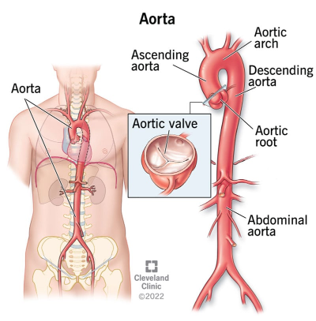
\includegraphics[width=0.4\textwidth]{figures/Intro/Aorta.png}
    \caption[Aorta]{Aorta}
    \label{fig_aorta}
\end{figure}

Aorta segmentation in computerized tomography (CT) scans is important for:
\begin{itemize}
\item Coarctation of the aorta
\item Aortic calcification quantification
\item To guide the segmentation of other central vessels. 
\end{itemize} ~\\

\subsection{Organ Segmentation}
The definition of the organ boundary or organ segmentation is helpful for the orientation and identification of the regions of interest inside the organ during the diagnostic or treatment procedure. Further, it allows the volume estimation of the organ, such as the aorta.

\begin{figure}[ht]
    \centering
    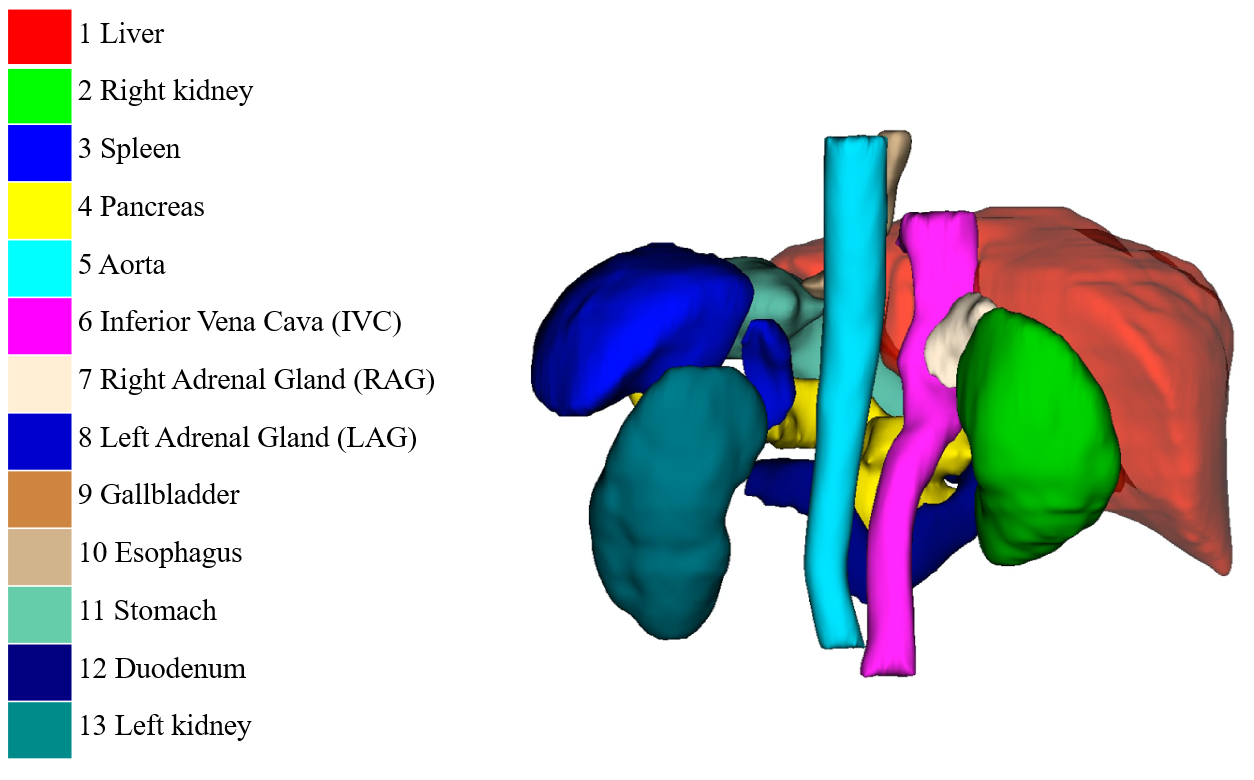
\includegraphics[width=0.7\textwidth]{figures/Intro/segmentation.png}
    \caption[Organ Segmentation]{Organ Segmentation \cite{Ma-2021-AbdomenCT-1K}}
    \label{fig_seg}
\end{figure}

\subsection{Assurance Case}

\begin{figure}[ht]
    \centering
    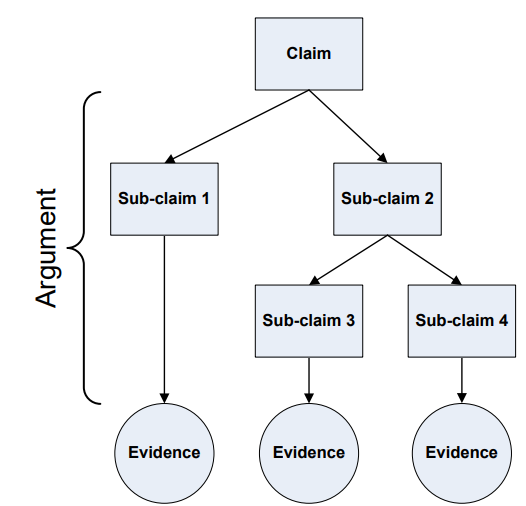
\includegraphics[width=0.45\textwidth]{figures/Intro/ac_diagram.png}
    \caption[Simple Assurance Case Diagram]{Simple Assurance Case Diagram \cite{doi:10.2514/6.2009-1921}}
    \label{fig_ac_diagram}
\end{figure}


An assurance case can be thought of as a specific type of argumentation used in various cases \cite{doi:10.2514/6.2009-1921}. When building an assurance case, you're essentially making a point that specific evidence backs up a particular statement. The fundamental structure is depicted in Figure \ref{fig_ac_diagram}. So, an assurance case essentially boils down to an organized collection of arguments, backed by a body of evidence, that helps validate the belief in a specific claim.

In a practical sense, creating an assurance case involves beginning with a main claim and then breaking it down into smaller claims through a step-by-step process. These smaller claims, at the most bottom, are supported by concrete evidence.


\section{Thesis Outline} \label{TO}

The thesis is organized into three broad parts. In Chapter 2, we introduce our program \progname{} by mentioning the existing methods, the AortaGeomRecon's algorithm overview and step by step  workflow. We explain necessary terms and information to understand how the software functionsfinally, and the 3D Slicer \cite{Kikinis2014} extension module that the user interacts with to get the segmentation result with our algorithm. In Chapter 3, we present our assurance case, some sections of our SRS, Design Documents, Module Guide, Algorithm Review, and a test case we developed for verifying and validating the correctness of program \progname{}. In Chapter 4, future work is proposed and conclusions are drawn based on the developed assurance case, SRS, segmentation algorithm and 3D Slicer module extension.